\documentclass[10pt,a4paper]{article}
\usepackage[latin1]{inputenc}
\usepackage{amsmath}
\usepackage{amsfonts}
\usepackage{amssymb}
\usepackage{graphicx}


\usepackage{hyperref}

%%% formatting the code
\usepackage{listings}



\usepackage{color}
\lstset{%
	escapeinside={(*}{*)},%
}

\newcommand{\amidstversion}{\input{../../version.txt}}

\lstset{
	frameround=fttt,
%	language=java,
	numbers=left,
	breaklines=true,
	mathescape, 
	columns=fullflexible, 
	basicstyle=\fontfamily{lmvtt}\selectfont,
	keywordstyle=\color{blue}\fontfamily{lmvtt}\selectfont, 
	numberstyle=\color{black}
}
\lstMakeShortInline[columns=fixed]|



\newcommand{\includejavasource}[1]{\lstinputlisting[language=java]{#1}}
\newcommand{\inlinejava}[1]{\lstinline[columns=fixed,language=java]{#1}}

\newcommand{\lang}[1]{}


\begin{document}
	
	\section{Loading AMIDST dependencies from a remote maven repository}








Here we explain how to add the AMIDST dependencies in a maven project with Java 8 or higher.  Alternatively, you might prefer following the video-tutorial in this \href{https://www.youtube.com/watch?v=i_X6cFo91LE}{link} .\newline

In this example, we will use a  project containing only one class, though the procedure here explain  could be used in any other maven project. You can check this \href{https://www.jetbrains.com/help/idea/2016.1/getting-started-with-maven.html}{link} for getting more information about how to create a new mavenproject.\newline

For using the AMIDST Toolbox, the \textbf{pom.xlm} file will be modified. First, in the Project view (located on the left) select the file pom.xml of your project and open it:\newline


\begin{figure}[h!]
	\centering 
	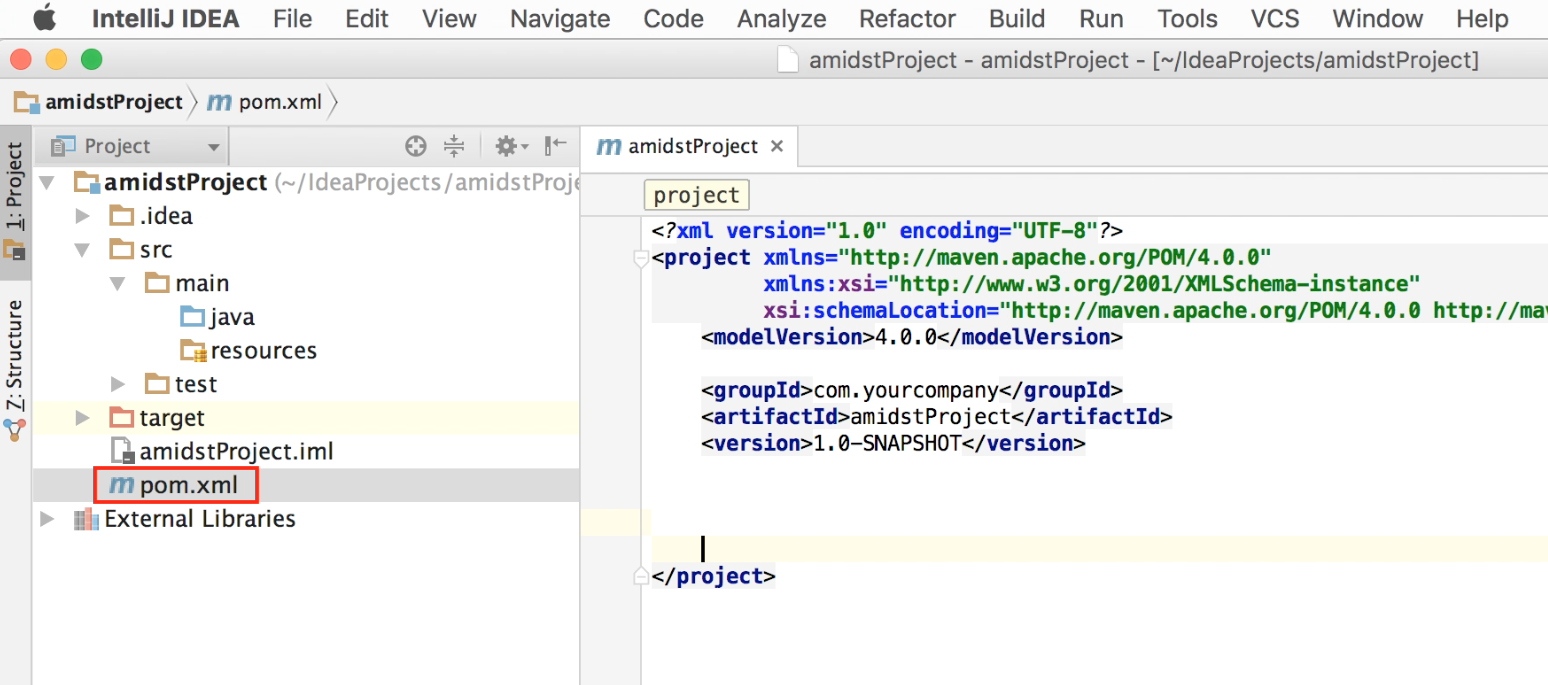
\includegraphics[width=8.5cm]{img/use_amidst05.png}
	\caption{Capture of Maven project in IntelliJ  and the initial pom.xml file}
	\label{fig:remoteDeps_initialPom}	
\end{figure}



\noindent Add the AMIDST repository by including the following code to your
pom:\newline

\begin{lstlisting}
<repositories>
<!-- AMIDST repository in github -->
<repository>
<id>amidstRepo</id> <!-- local identifier, it can be anything -->
<url>https://raw.github.com/amidst/toolbox/mvn-repo/</url>
</repository>
<!-- ... -->
</repositories>        
\end{lstlisting}



Then, add the dependencies of modules in AMIDST you want to use.~
For each module, add an element \textbf{\textless{}dependency\textgreater{}\textbf{\ldots{}\textless{}/dependency\textgreater{}}}
inside the labels
\textbf{\textless{}dependencies\textgreater{}\textless{}/dependencies\textgreater{}}. For each one, we have to indicate the following
information:\newline

\begin{itemize}
	\item
	\textbf{groupId} is an identifier of the project's module. In this case it
	should containt the value \emph{``eu.amidst''.}
	\item
	\textbf{artifactId }is the name of the module we want to use. More precisely,
	it is the name of the jar file containing such module. You can see the
	list of AMIDST modules
	\href{https://github.com/amidst/toolbox/tree/mvn-repo/eu/amidst}{here}.
	\item
	\textbf{version} is the identifier of~ AMIDST Toolbox release. You can
	see
	\href{mohttps://github.com/amidst/toolbox/blob/master/CHANGELOG.mddules\%20here}{here}
	the list of all versions available.
	\item
	\textbf{scope}~ allows you to only include dependencies appropriate
	for the current stage of the build. We will set this to
	\emph{``compile''.}
\end{itemize}


\vspace{2mm}
\noindent For example, for using the \textit{core-dynamic }module, include the
following code:

\begin{lstlisting}
<dependencies>
<!-- Load any of the modules from AMIDST Toolbox -->
<dependency>
<groupId>eu.amidst</groupId>
<artifactId>core-dynamic</artifactId>
<version>(*\amidstversion*)</version>
<scope>compile</scope>
</dependency>

<!-- ... -->
</dependencies>        
\end{lstlisting}

Note that for using another module,  simply change the value of the
element artifactId (i.e. the content between the tags
\textless{}artifactId\textgreater{} and
\textless{}artifactId\textgreater{}). Now you can check in the \textbf{Maven Projects panel }that all the
dependencies have been loaded:\newline 


\begin{figure}[h!]
	\centering
	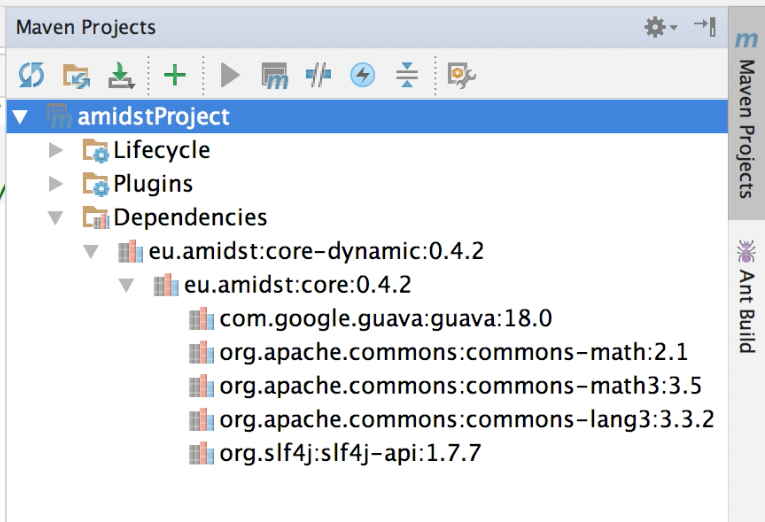
\includegraphics[width=8.5cm]{img/use_amidst07.png}
	\caption{List of loaded dependencies}
	\label{fig:remoteDeps_mavenPanel}	
\end{figure}


\newpage 

Note that the \emph{core-dynamic module} depends on {core }{}that has
been loaded as well. We recomend you to download the sources and the
javadoc:



\begin{figure}[h!]
	\centering
	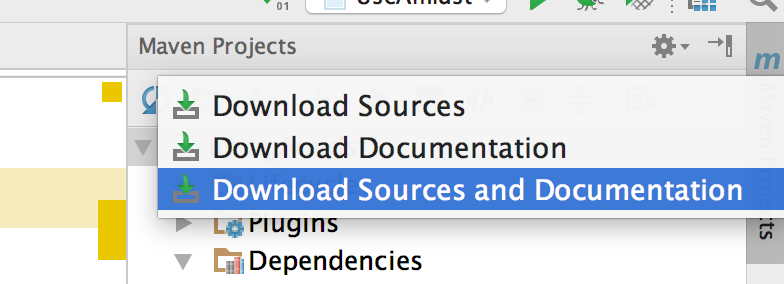
\includegraphics[width=10cm]{img/use_amidst08.png}
	\caption{Download the JavaDoc and  the source code}
	\label{fig:remoteDeps_downloadJD}	
\end{figure}




Finally, for testing purposes, we can run the code shown below that generates a random dynamic bayesian network (DBN) and prints its parameters.

\begin{verbatim}
import eu.amidst.dynamic.models.DynamicBayesianNetwork;
import eu.amidst.dynamic.utils.DynamicBayesianNetworkGenerator;

public class TestingAmidst {
  public static void main(String[] args) throws WrongConfigurationException {
    DynamicBayesianNetworkGenerator.setNumberOfContinuousVars(2);
    DynamicBayesianNetworkGenerator.setNumberOfDiscreteVars(5);
    DynamicBayesianNetworkGenerator.setNumberOfStates(3);

    DynamicBayesianNetwork extendedDBN = 
    DynamicBayesianNetworkGenerator.generateDynamicBayesianNetwork();    

    System.out.println(extendedDBN.toString());


  }

}

\end{verbatim}

\noindent If everything goes right, the following output will be
generated:\newline


\begin{figure}[h!]
	\centering
	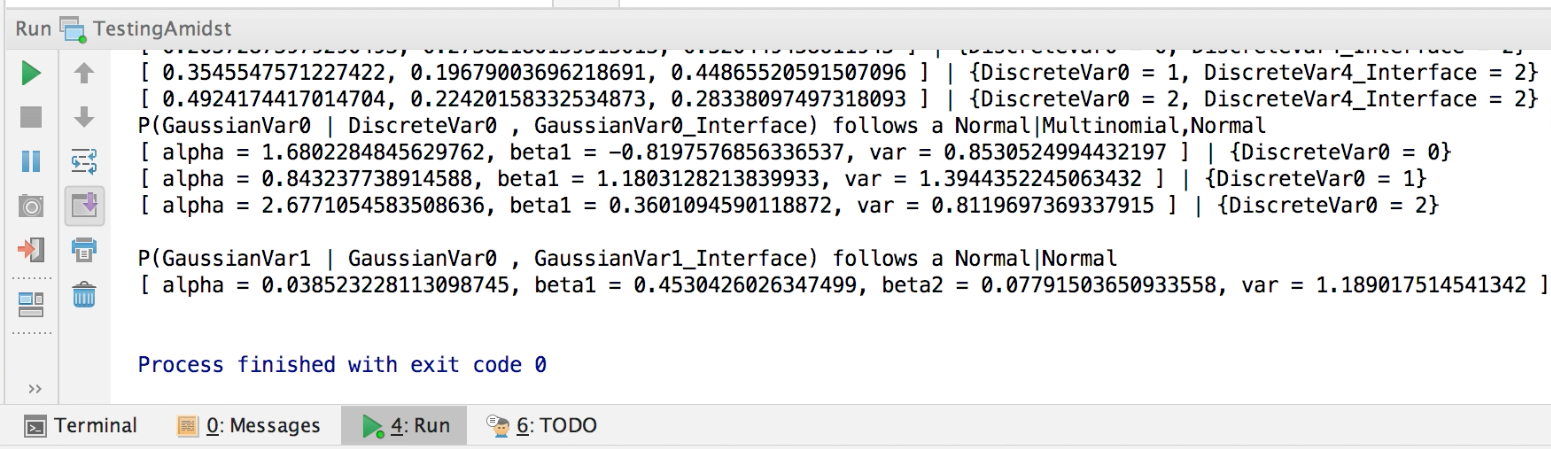
\includegraphics[width=8.5cm]{img/use_amidst09.png}
	\caption{Ouput of the testing code that generates a random  DBN}
	\label{fig:remoteDeps_output}	
\end{figure}



\end{document}